% \iffalse meta-comment
% This is file `seuthesix.dtx',
% This file provides a LaTeX document class for typesetting thesis of Southeast University, Nanjing, China.
% Copyright (c) 2007--2012 Xu Yuan, email: xuyuan.cn@gmail.com
% Copyright (c) 2016 James Fan, email: zhimengfan1990@163.com
% License: GNU General Public License, version 3
%This file is part of ``seuthesix'' package.
%``seuthesix'' is free software: you can redistribute it and/or modify
%it under the terms of the GNU General Public License as published by
%the Free Software Foundation, either version 3 of the License, or
%(at your option) any later version.
%``seuthesix'' is distributed in the hope that it will be useful,
%but WITHOUT ANY WARRANTY; without even the implied warranty of
%MERCHANTABILITY or FITNESS FOR A PARTICULAR PURPOSE.  See the
%GNU General Public License for more details.
%
%You should have received a copy of the GNU General Public License
%along with this program.  If not, see <http://www.gnu.org/licenses/>.
%
% \fi
%
% \iffalse
%<*driver>
\ProvidesFile{seuthesix.dtx}
%</driver>
%<*driver>
[2016/01/15 1.0.1 The LaTeX template for academic  degree thesis of Southeast University]
%</driver> 
%
%<*driver>
\documentclass[figurelist,tablelist,algorithmlist,nomlist,masters]{seuthesix}
\usepackage{doc}
\usepackage{hologo}
\usepackage{pdfpages}
\CodelineNumbered
\GetFileInfo{skeleton.dtx}
\DoNotIndex{\newcommand,\newenvironment,\def}
\begin{document}
\DocInput{seuthesix.dtx}
\end{document}
%</driver>
%
% \fi
%
% \CheckSum{0}
%
% \CharacterTable
%  {Upper-case    \A\B\C\D\E\F\G\H\I\J\K\L\M\N\O\P\Q\R\S\T\U\V\W\X\Y\Z
%   Lower-case    \a\b\c\d\e\f\g\h\i\j\k\l\m\n\o\p\q\r\s\t\u\v\w\x\y\z
%   Digits        \0\1\2\3\4\5\6\7\8\9
%   Exclamation   \!     Double quote  \"     Hash (number) \#
%   Dollar        \$     Percent       \%     Ampersand     \&
%   Acute accent  \'     Left paren    \(     Right paren   \)
%   Asterisk      \*     Plus          \+     Comma         \,
%   Minus         \-     Point         \.     Solidus       \/
%   Colon         \:     Semicolon     \;     Less than     \<
%   Equals        \=     Greater than  \>     Question mark \?
%   Commercial at \@     Left bracket  \[     Backslash     \\
%   Right bracket \]     Circumflex    \^     Underscore    \_
%   Grave accent  \`     Left brace    \{     Vertical bar  \|
%   Right brace   \}     Tilde         \~}
%\changes{v1.0.1}{2016/01/15}{using \texttt{doc} to package source into \texttt{.dtx}}
%\changes{v1.0}{2016/01/09}{initial version}
%\categorynumber{000} 
%\UDC{000}            
%\secretlevel{公开}   
%\studentid{000000}   
%\title{\seuthesix 用户手册}{手册}{\seuthesix User Manual}{\seuthesix}
%\author{\seuthesix 开发组}{\seuthesix developer group}
%\advisor{高德纳}{教授}{Donald E. Knuth}{Prof.}
%\coadvisor{兰伯特}{副教授}{Leslie Lamport}{Associate Prof.} 
%\degreetype{\TeX 学硕士}{Master of \TeX}
%\major{\TeX}
%\submajor{\LaTeX}
%\defenddate{\today}
%\authorizedate{\today}
%\committeechair{高德纳}
%\reviewer{Frank Mittlebach}{David Carlisle}
%\department{\TeX{}学院}{School of \TeX}
%\seuthesisthanks{本课题的研究获\LaTeX{ }project 赞助\url{www.latex-project.org}}
%\makebigcover
%\makecover
%\begin{abstract}{\TeX, \LaTeX, 文档类, 学位论文}
%本文介绍如何使用\seuthesix 文档类撰写东南大学学位论文。
%\end{abstract}
%\begin{englishabstract}{\TeX, \LaTeX, document class, thesis/dissertation}
%This work presents an introduction of how to use \seuthesix document class to 
%typeset the thesis/dissertation of Southeast University.
%\end{englishabstract}
%
%\tableofcontents
%\listofothers
%
%\mainmatter
%\chapter{绪论}
% \verb+seuthesix.cls+ 提供了符合规范的东南大学硕士与博士学位论文的\LaTeX 模板。
% 模板的格式尽量满足东南大学研究生院和教务处的要求,当然由于水平有限其中错
% 漏在所难免,我们欢迎东大的 \LaTeX{er} 一起参加开发和完善。如果您对开发和完善\seuthesix
% 感兴趣、有任何想法或建议,请与我们联系。该项目主页GitHub:
% \url{https://github.com/zhimengfan1990/seuthesix}。
%
% 本模板基于早期许元同学发布的\verb+seuthesis.cls+。由于其中出现不少bug,无法顺利通过编译,
% 因此决定进行修改。由于修改内容较大,最终决定单独发布一个新的package。为了表示两者的继承关系,
% 新的package 取名为\seuthesix, 即\seuthesis{ }eXtented version。\seuthesix 初始版本号定为1.0。
%
% \section{版权声明}
% \begin{tabular}{ll}
% 版权所有\copyright 2007--2012 & 许 元 (\url{xuyuan.cn@gmail.com})\\
% &宋翊涵 (\url{syhannnn@gmail.com})\\
% & 黄小雨 (\url{nobel1984@gmail.com})\\
% 版权所有\copyright 2016 & 樊智猛 (\url{zhimengfan1990@163.com})
% \end{tabular}
% \par
% 这一程序是自由软件,你可以遵照自由软件基金会发布的《GNU 通用公共许可证
% 条款第三版》来修改和重新发布这一程序,或者 (根据您的选择) 用任何更新的版本。
% 发布这一程序的目的是希望它有用,但没有任何担保。甚至没有适合特定目的的隐含
% 的担保。更详细的情况请参阅《GNU 通用公共许可证》
% \footnote{\url{http://www.gnu.org/licenses/gpl.html}}
%
% \section{版本历史}
% \begin{description}
% \item[1.0] 2016/01/11,基于\seuthesis 构建新的\seuthesix 文档类。放弃\seuthesis 
% 的xeCJK方案 ,直接采用\verb+ctexrep.cls+ 构建\verb+seuthesix.cls+。
% 重新编写参考文献格式\verb+seuthesix.bst+。一次性生成A3大封面、A4封面和论文内容,简化了操作。
%放弃对本科学位论文的支持(精力有限)。
% \end{description}
%
% \chapter{下载和安装}
% \section{下载}
% 本项目最新源码可以到本项目在 GitHub 中找到,访问
% \url{https://github.com/zhimengfan1990/seuthesix}下载。各发布版本可在\LaTeX 官方 CTAN: 
% \url{http://www.ctan.org/pkg/seuthesix}下载。
% \section{安装}
% 将宏包中的文件放在当前工作目录(与 \verb+.tex+ 文件放在同一目录下)即可。
% 当然也可以安装到 \TeX 系统
% 中,不过需要注意是参考文献样式文件 \verb+.bst+ 必须置于 \verb+TEXMF/bibtex/bst+ 目录或子目
% 录下。但是,不建议手工安装到\TeX 系统中。一般可以借助某些工具来完成安装。如使用的是\TeX Live, 
%只需要在命令行执行\\
%\verb+tlmgr install seuthesix+\\
%即可。
%
% 本模板在 \TeX{Live} 2015(Windows 7 和 LinuxMint 17.1 环境下) 通过\hologo{XeLaTeX} 编译通过。
% 如有您在使用中有任何问题,欢迎与我联系。
%
%\newgeometry{left=4cm,right=4cm,textwidth=13cm}
% \chapter{使用说明}
% 学位论文应包括如下部分:\\
% \begin{enumerate}
% \itshape
% \item 中文封面
% \item 中文页面
% \item 英文页面
% \item 论文独创性声明和使用授权声明
% \item 中文内容提要及关键词
% \item 英文内容提要及关键词
% \item 目录
% \item \fbox{符号、变量、缩略词等本论文专用术语的注释表}
% \item 正文
% \item \fbox{致谢}
% \item 参考文献
% \item  \fbox{附录}
% \item \fbox{索引(中、英文)}
% \item  \fbox{作者简介(包括在学期间发表的论文和取得的学术成果清单)}
% \item \fbox{后记}
% \end{enumerate}
% 并按此顺序排列,其中\fbox{加方框的条目}为可选。
%
%\section{模板整体框架}
%使用 \seuthesix 模板的整体框架如下所示,其中\verb+<...>+表示可替换的文本(replaceable text)。
%{\color{magenta}
%\begin{verbatim}
%\documentclass[figurelist,tablelist,algorithmlist,nomlist,masters]{seuthesix}
% %文档开始,指定选项
%\usepackage{<hologo>}
%\usepackage{<pdfpages>}%载入更多宏包
%
%\categorynumber{<000>} % 分类采用《中国图书资料分类法》
%\UDC{<000>}            %《国际十进分类法UDC》的类号
%\secretlevel{<公开>}    
% %学位论文密级分为"公开"、"内部"、"秘密"和"机密"四种
%\studentid{<000000>}   %学号要完整,前面的零不能省略。
%\title{<\seuthesix 用户手册>}{<手册>}{<\seuthesix User Manual>}{<\seuthesix>}
% %中文标题,中文副标题,英文标题,英文副标题, 副标题没有可以置为空, 
% %即 \title{<\seuthesix 用户手册>}{}{<\seuthesix User Manual>}{}
%\author{<\seuthesix 开发组>}{<\seuthesix developer group>}
% %作者中英文姓名
%\advisor{<高德纳>}{<教授>}{<Donald E. Knuth>}{<Prof.>}
% %导师中英文姓名与职称
%\coadvisor{<兰伯特>}{<副教授>}{<Leslie Lamport>}{<Associate Prof.>} 
% %副导师中英文姓名与职称,若没有,可以不使用该命令
% \degreetype{<\TeX 学硕士>}{<Master of \TeX>} 
% %详细学位类型,如工学硕士,Master of Engineering
%\major{<\TeX>}%一级学科名
%\submajor{<\LaTeX>}%二级学科名
%\defenddate{<\today>}%答辩日期
%\authorizedate{<\today>}%授予学位日期
%\committeechair{<高德纳>}%答辩委员会主席姓名
%\reviewer{<Frank Mittlebach>}{<David Carlisle>}%两位评阅人姓名
%\department{<\TeX{}学院>}{<School of \TeX>}
% %学院名称
%\seuthesisthanks{<本课题的研究获\LaTeX{ }project 赞助\url{www.latex-project.org}>}
% %致谢信息,没有可以不写
%\makebigcover%生成A3大封面
%\makecover% 生成封面
%\begin{abstract}{<\TeX, \LaTeX, 文档类, 学位论文>}
% <本文介绍如何使用\seuthesix 文档类撰写东南大学学位论文。>
%\end{abstract}
% %生成中文摘要和关键词
%\begin{englishabstract}{<\TeX, \LaTeX, document class, thesis/dissertation>}
% <This work presents an introduction of how to use \seuthesix document class to 
% typeset the thesis/dissertation of Southeast University.>
%\end{englishabstract}
% %生成英文摘要和关键词
%\tableofcontents%生成目录
%\setnomname{<术语表名称>}%设置术语表的名称,用于\listofothers
%\listofothers%生成图、表等目录,没有可以不写
%
%\mainmatter
% %开始正文
%
%\chapter{<绪论>}
%\section{<研究背景>}
%\section{<本论文的工作>}
%...
%
%
%\chapter{<...>}
%\section{<...>}
%...
%
%
%...
%
%
%\chapter{<全文总结>}
%...
%
%\acknowledgement
% <感谢每一个给予帮助的人...>
% %致谢,没有可以不写
%
%\thesisbib{<bib文件名>}
% %参考文献
%
%\appendix
%\chapter{<...>}
%...
%
%\chapter{<...>}
%...
% %附录部分,没有可以不写
%
%\resume{<作者简介>}
% <简介内容...>
% %作者简介,没有可以不写
%
%\end{document}
% %文档到此结束
%\end{verbatim}
%}
%\section{详细说明}
%下面对这些命令及其参数进行详细介绍。注意,为使得代码能够正常显示在边缘,本章及后续的page layout 有所改变,
%但这种改变在
%正常的论文中是不会出现的。
%\DescribeMacro{\documentclass}\DescribeMacro{masters}\DescribeMacro{phd}\DescribeMacro{engineering}
% 该命令使用\texttt{seuthesix}文档类,其中用\texttt{masters, phd, engieering} 来分别表示
% 学术硕士,博士,和工程硕士的学位论文。三者的区别主要在于封面的logo 不同。此外,
% 博士学位论文称为Dissertation, 而硕士学位论文(包括学术型和工程硕士)称为Thesis 。
% 例如,学术型硕士应该是\verb+\documentclass[masters]{seuthesix}+。默认为\texttt{masters}。
%
%\DescribeMacro{nocolorlinks}
% 除了这三项之外,还可以添加别的选项。如{\texttt{nocolorlinks}}用于最终论文付梓(打印)时去除
% \texttt{hyperref}宏包。产生的颜色链接(用方框表示,但该方框在打印时无效),使得打印的纸质版在这些地方更清晰。
%\DescribeMacro{figurelist}\DescribeMacro{tablelist}\DescribeMacro{algorithmlist}\DescribeMacro{nomlist}
%\DescribeMacro{\listofothers}
%如果需要在目录之后产生插图目录、表格目录、算法目录、术语与符号目录,需要分别
% 提供\texttt{figurelist, tablelist, algorithmlist, nomlist}选项来指定。若这四个目录中至少有一个,
% 还需要给出\verb+\listofothers+命令来真正将该表格排版出来。
% 若四个目录都不需要,则无需给出这四个选项和\verb+\listofothers+命令。
% 此外,基本参数,如纸张大小,页面布局等已经在文档类中指定,用户无需再次指定。
% 对于Windows 系统,系统默认编码方式为GBK,因此需要注意使用
% 编辑器将源文件以UTF8 编码保存,否则会出现乱码。对于Linux,系统默认编码就是UTF8,因此不存在这个问题。
%
%\DescribeMacro{\usepackage}
% 如果用户还需要载入更多的宏包,可以通过这个命令载入。但是前提是不能破坏\seuthesix 文档类的基本参数设定。
% 一般来讲,是不需要载入其他宏包的,除非用户知道自己到底在干什么。
%
% 为了生成封面,需要用户提供一些基本信息。
%
%\DescribeMacro{\categorynumber} \verb+\categorynumber{<cat_number>}+用于提供分类号。
%
%\DescribeMacro{\UDC} \verb+\UDC{<udc>}+ 用于提供UDC。
%
%\DescribeMacro{\secretlevel} \verb+\secretlevel{<level>}+ 用于提供密级。
%
%\DescribeMacro{\studentid}\verb+\studentid{<id>}+用于提供学号,6位数,前导0不能省略。
%
%\DescribeMacro{\title}\verb+\title{<ch_title>}{<ch_subtitle>}{<en_title>}{<en_subtitle>}+四个参数分别提供
%中文标题,中文副标题,英文标题,英文副标题。若不需要副标题,可将其置为空。例如没有中文和英文副标题,则可简化为
%\verb+\title{<ch_title>}{}{<en_title>}{}+。
%
%\DescribeMacro{\author}\verb+\author{<ch_name>}{<en_name>}+提供作者姓名中英文姓名。
%
%\DescribeMacro{\advisor}\verb+\advisor{<ch_name>}{<ch_title>}{<en_name>}{<en_title>}+用于提供导师中文姓名,
%中文职称,英文姓名,英文职称。如\verb+\advisor{张三}{教授}{Zhang San}{Prof.}+。
%
%\DescribeMacro{\coadvisor}\verb+\coadvisor{<ch_name>}{<ch_title>}{<en_name>}{<en_title>}+用于提供副导师中文姓名,
%中文职称,英文姓名,英文职称。如\verb+\coadvisor{李四}{副教授}{Lee Si}{Associate Prof.}+。该命令可以不用,当没有副导师
%时,无需使用该命令。
%
%\DescribeMacro{\degreetype}\verb+\degreetype{<ch_type>}{<en_type>}+ 用于提供中英文的学位类型。如
%\verb+\degreetype{工学硕士}{Master of Engineering}+。
%
%\DescribeMacro{\major} \verb+\major{<mjr>}+ 用于提供一级学科名称,如信息与通信工程。
%
%\DescribeMacro{\submajor}\verb+\submajor{<sub_mjr>}+ 用于提供二级学科名称,如通信与信息系统。
%
%\DescribeMacro{\defenddate}\verb+\defenddate{<YYYY 年 MM 月 dd 日>}+ 用于提供答辩日期,包括年、月、日。
%
%\DescribeMacro{\authorizedate}\verb+\authorizedate{<YYYY 年 MM 月 dd 日>}+ 用于提供学位授予日期。
%
%\DescribeMacro{\committeechair}\verb+\committeechair{<name>}+ 用于提供答辩委员会主席的姓名(中文)。
%
%\DescribeMacro{\reviewer} \verb+\reviewer{<name_A>}{<name_B>}+ 用于提供两位评阅人的中文姓名。
%
%\DescribeMacro{\department}\verb+\department{<dpt_name>}+ 用于提供学院名称,如信息科学与工程学院。
%
%\DescribeMacro{\seuthesisthanks}\verb+\seuthesisthanks{<thanks_words>}+ 用于提供致谢语,一句话。
%将会出现在中文封面页脚处。如\verb+\seuthesisthanks{本课题的研究受国家高技术发展计划(863计划)2016XXXXXX 资助}+。
%若没有,可以不使用该命令。
%注意,这不是论文末尾处的致谢章。
%
%\DescribeMacro{\makebigcover}
%提供了相关信息之后,就可以利用这条命令来生成A3大封面。
%
%\DescribeMacro{\makecover}
%这条命令生成A4中文封面和英文封面。
%
%\DescribeEnv{abstract}
%\begin{verbatim}
%\begin{abstract}{<ch_keywords>}
%...
%\end{abstract}
%\end{verbatim}
%这个环境用于生成中文摘要。该环境带一个参数,即中文关键词,关键词为逗号分隔表(comma seperated list)的形式。
%
%\DescribeEnv{englishabstract}
%\begin{verbatim}
%\begin{englishabstract}{<en_keywords>}
%...
%\end{englishabstract}
%\end{verbatim}
%这个环境用于生成英文摘要。该环境带一个参数,即英文关键词,关键词为逗号分隔表(comma seperated list)的形式。
%
%\DescribeMacro{\setnomname}
%\verb+\setnomname{<name>}+ 用于设置术语表的名称,如“术语与数学符号约定”。该命令用于生成术语表。如不需要术语表,
%则不用使用该命令。
%
%\DescribeMacro{\tableofcontents}
%该命令用于生成目录。
%
%\DescribeMacro{\listofothers}
%该命令用于生成插图目录,表格目录,算法目录,术语目录(术语表)。插图目录、表格目录、算法目录名称都是固定的。
%术语目录名称考虑到不同学科有差异,可通过\verb+\setnomname{<name>}+进行设置。
%同时,该命令最终会生成四个目录中的哪几个是通过文档类的选项来指定的,前文已经讲过。
%
%\DescribeMacro{\mainmatter}
%该命令切换到正文状态。页码从阿拉伯数字1开始,此前页码为罗马数字形式。
%给出以上命令之后,就可以开始正文章节的内容。正文章节遵循普通\LaTeX 的语法规则即可。
%
%完成正文章节之后,开始致谢、参考文献、附录、作者简介等。
%
%\DescribeMacro{\acknowledgement}
%该命令开启一个新的章(没有章编号),之后用户可以写入致谢内容。致谢内容自成一章。
%该部分可选。
%
%\DescribeMacro{\thesisbib}
%\verb+\thesisbib{<filename>}+该命令用于生成参考文献,采用\hologo{BibTeX}工具自动生成。
%为此,用于需提供\texttt{.bib}数据库文件名称作为该命令的参数,不需要包含扩展名。
%
%\DescribeMacro{\appendix}
%该命令切换到目录状态。
% 此后的每个\verb+\chapter{<...>}+都会变成一个附录。
% 章编号变为“附录A,附录B”,等等。
% 该部分及后续的附录章为可选。
%
%\DescribeMacro{\resume}
%\verb+\resume{<title>}+ 该命令用于生成作者简历,自成一章。通过该命令 的参数提供该章
%的标题。简历的具体内容由用户输入。该部分可选。
%
%\restoregeometry
%从此处开始,恢复标准论文模板的page layout。
% \chapter{注意事项}
% \section{文献引用}
% 根据要求,文献引用应为数字标签(numerical label),上标形式。但是有时也会用到正常形式,即非
% 上标形式,用于正文叙述。为此分别提供了两个命令来实现。
% \begin{verbatim}
% \cite{<citation_key>}
% \end{verbatim}
% 用于实现上标的数字形式文献引用\cite{knuth},
% \begin{verbatim}
% \citen{<citation_key>}
% \end{verbatim}
% 用于实现正常(非上标,normal)的数字形式文献引用\citen{mittlebach}。
% \section{参考文献格式}
% 见\verb+seuthesix.bst+的文档: 本文第\ref{bst}章。
%
% \section{图表格式处理}
% 图名、表名字体字号已经有文档类 设定好,用户无需再次设定。但是,用户需要让它居中。图名位于图下方,
% 表名位于表上方。图片文件可直接置于当前工作目录,也可置于当前工作目录的\texttt{figures}子目录下(用户根据需要,自己创建该子目录)。
% 图片名称只需要给出名称和扩展名,无需给出完整的路径。图\ref{logo}给出了一个图的例子。表\ref{entrytable}给出了一个表的例子。
% 
% \begin{verbatim}
% \begin{figure}
% \centering
% \includegraphics[...]{...}
% \caption{...}
% \label{...}
% \end{figue}
% ...
% \begin{table}
% \centering
% \caption{...}
% \label{...}
% \begin{tabular}{...}
% ...
% \end{tabular}.
% \end{table}
%
% \end{verbatim}
% 
%
% \begin{figure}
% \centering
% \caption{\seuthesix logo\label{logo}}
% \chuhao \seuthesix
% \end{figure}
%
% \section{算法格式处理}
% \seuthesix 文档类采用了\texttt{algorithm, algorithmic }两个宏包来设置算法排版格式。
% 详细使用方法参见这两个宏包的手册。这里给出一个简单的例子。
% 
% \begin{verbatim}
% \begin{algorithm}
% \caption{\label{algoinsight}如何使用\seuthesix 文档类}
% \begin{algorithmic}[1]
% \STATE if (具备一定的\LaTeX 使用经验) else (stop here)
% \STATE 有耐心阅读文档
% \STATE 仔细阅读本文档
% \STATE 在使用中熟悉它
% \end{algorithmic}
% \end{algorithm}
% \end{verbatim}
% 
%
% 以上代码给出了算法\ref{algoinsight}的排版结果。
% \begin{algorithm}
% \caption{\label{algoinsight}如何使用\seuthesix 文档类}
% \begin{algorithmic}[1]
% \STATE if (具备一定的\LaTeX 使用经验) else (stop here)
% \STATE 有耐心阅读文档
% \STATE 仔细阅读本文档
% \STATE 在使用中熟悉它
% \end{algorithmic}
% \end{algorithm}
%
% \section{术语生成}
% \begingroup
% \begin{verbatim}
% \nomenclature{LTE}{Long Term Evolution}
% \nomenclature[noprefix]{$\mathcal{CN}(0, C)$}{协方差矩阵为$C$的循环对称复高斯分布}
% \end{verbatim}
% \endgroup
%
% \nomenclature{LTE}{Long Term Evolution}
% \nomenclature[noprefix]{$\mathcal{CN}(0, C)$}{协方差矩阵为$C$的循环对称复高斯分布}
% 术语生成借助\texttt{nomencl}宏包。以上代码例子的排版结果在术语表中。对于数学符号,为使得它
% 排在普通术语的后面,需要加上\texttt{[noprefix]}选项。
% 编译时,第一次
%
% \verb+xelatex <filename>+ 
%
% 之后执行 
%
% \verb+makeindex <filename> .nlo -s nomencl.ist -o <filename> .nls+
%
% 然后再次执行
%
% \verb+xelatex <filename>+
%
% 一次。实际上,考虑到参考文献的生成,最后应该执行
%
% \verb+xelatex <filename>+
%
% 至少两次。
%
% \chapter{\texttt{seuthesix.bst}参考文献格式\label{bst}}
% \section{简介}
% \texttt{seuthesix.bst} 是符合东南大学硕士和博士毕业论文参考文献格式要求的 bibliography style。
% 由于该文献格式是数字标签(numeric label)格式,且无需排序。因此,它是在标准的BibTeX
% 格式\texttt{unsrt.bst} 的基础上发展而来。同时,\verb=seuthesix.bst=文献格式不支持\texttt{crossref}字段。
% 该文献格式支持中英文两种语言,采用中英文分离,分别进行处理的思想。对于中文文献的entry,
% 要求在\verb=.bib=文献数据库中该entry 提供\texttt{language} field
% ,其取值任意,但为了保持一致性,建议设为\verb+language={zh}+,或\verb+language="zh"+。
%
% \section{支持的Entry type}
% \texttt{seuthesix.bst}支持以下几种不同的entry type。
% \begin{description}
% \item[book] 书籍
% \item[article] 期刊文章
% \item[inproceedings/conference] 会议文章
% \item[mastersthesis] 硕士学位论文
% \item[phdthesis] 博士学位论文
% \item[patent] 专利
% \item[standard] 标准
% \item[news] 报纸新闻
% \item[misc] 杂项,包括电子媒体及其他未能识别的entry type
% \end{description}
%
% \section{各 entry type 所支持的field}
% 不同的entry type所支持的field 不尽相同。对于每个entry type 而言,其中的field 可分为三类:
% required, optional, ignored。required field 应该必须出现,否则BibTeX 会发出warning(由bst中的output.check函数发出),
% 且最终得到的格式不能保证美观。
% optional field 可选,若未出现,不会导致BibTeX warning。ignored field 
% 不起任何作用,被BibTeX 忽略。在entry type 对应的bibtex 函数(如 \verb=FUNCTION {article}=)中未使用的 field 都属于 ignored field。
%
% 下面列出各entry type所支持的field(即required field 和optional field),
% 其中required field使用黑体。如表\ref{entrytable}所示。
%
% \begin{table}
% \centering
% \caption{\label{entrytable}不同entry type支持的field}
% \begin{tabular}{|c||p{10cm}|}
% \hline
% \bfseries Entry type & \raggedright\bfseries Fields\tabularnewline
% \hline\hline
% article & \raggedright{\bfseries author, title, journal, year, } volume, number, pages, note, {{\bfseries lang}uage}\tabularnewline
% \hline
% book & \raggedright{\bfseries author/editor, title, }edition, translator, address, publisher, year, pages, note, {{\bfseries lang}uage}\tabularnewline
% \hline
% inproceedings(conference) & \raggedright {\bfseries author, title, }editor, booktitle, address, publisher,
% year, pages, note, {{\bfseries lang}uage}\tabularnewline
% \hline
% mastersthesis  &\raggedright{\bfseries author, title, address, school, year, }note, {{\bfseries lang}uage}\tabularnewline
% \hline 
% phdthesis  &\raggedright{\bfseries author, title, address, school, year, }note, {{\bfseries lang}uage}\tabularnewline
% \hline 
% patent & \raggedright{\bfseries applicant\footnotemark, title, }littype\footnotemark,
% country, pid\footnotemark, year, month, day, 
% note, {{\bfseries lang}uage}\tabularnewline
% \hline
% standard & \raggedright{\bfseries author, title, }stdcode\footnotemark, address, publisher, year, 
% note, {{\bfseries lang}uage}\tabularnewline
% \hline
% news & \raggedright{\bfseries author, title, newspaper, }year, month, day, pages, note, {{\bfseries lang}uage}\tabularnewline
% \hline
% misc &\raggedright{\bfseries }author, title, url, year, month, day, note, {{\bfseries lang}uage}\tabularnewline
% \hline
% \end{tabular}
% \end{table}
% \footnotetext[1]{专利申请人}
% \footnotetext[2]{专利文献类型}
% \footnotetext[3]{专利号}
% \footnotetext[4]{标准号}
% 需要注意的是,若为英文参考文献,则language field 可以省略,而对于中文参考文献language field 则必须出现在\verb=.bib= 文献数据库中。
% 其取值任意,但建议设为\verb+language={zh}+,或\verb+language="zh"+,以保持一致性。
% 这就是表\ref{entrytable}中的{{\bfseries lang}uage}一半黑体一半非黑体的原因。
% 参考文献部分给出了很多文献格式的例子。
%
% \nocite{komine2004fundamental}
% \nocite{dimitrov2015principles}
% \nocite{fujimoto2014fastest}
% \nocite{ieee2012ieee}
% \nocite{irdawebsite}
% \nocite{vlcnews}
% \nocite{pt}
% \nocite{thesis:a}
% \nocite{thesis:b}
%
% \chapter{全文总结}
% 本文主要介绍了如何使用\seuthesix \LaTeX 文档类来对东南大学硕士与博士学位论文进行排版。
% 当然,\seuthesix 肯定存在许多不足的地方,希望各位读者予以指正。
%
% \acknowledgement
% 感谢每一个支持\seuthesix 的人。
%
% \thesisbib{seuthesix}
%
% \appendix
% \chapter{东南大学研究生学位论文的格式规定}
% 见下一页。
% 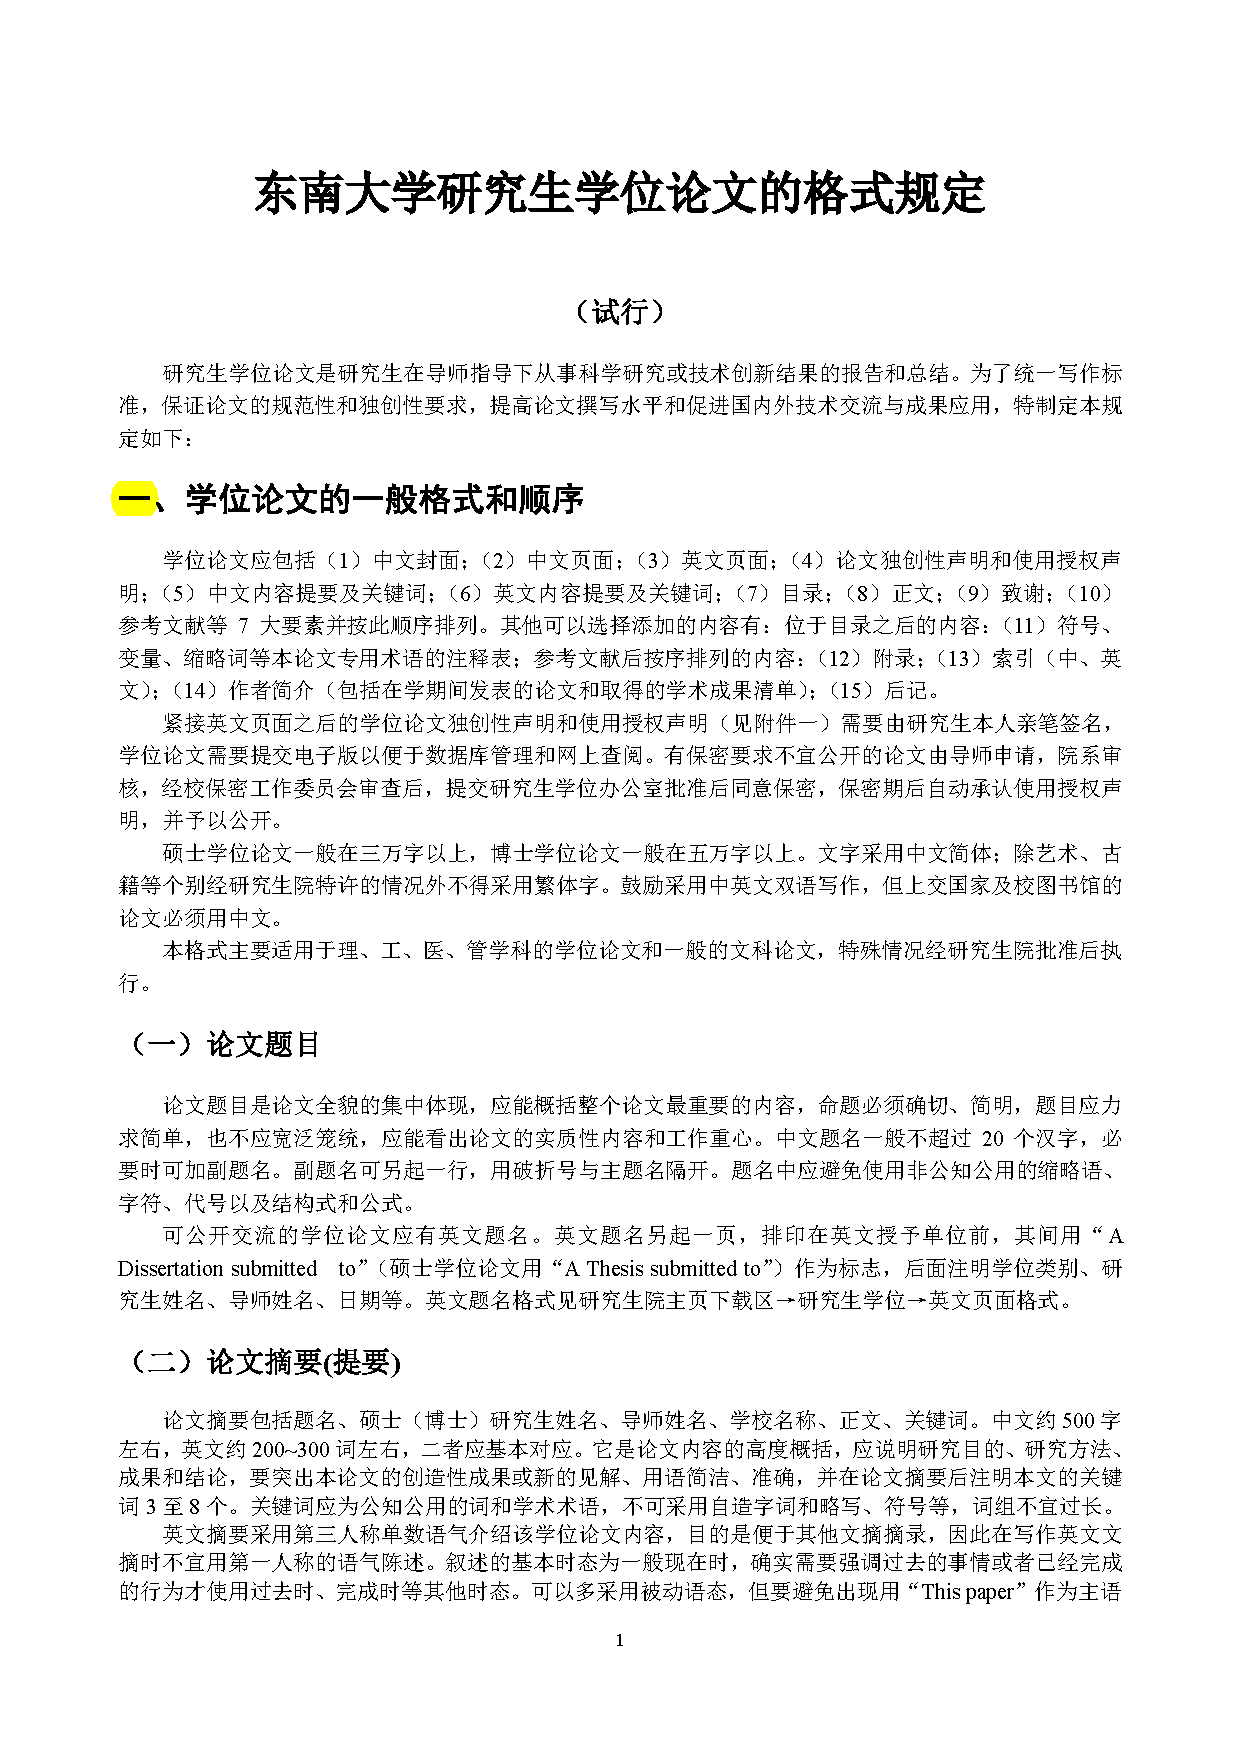
\includepdf[pages=-,fitpaper]{rules.pdf}
%\StopEventually{}
%\chapter{实现代码}
%    \begin{macrocode}
%<*class>
\NeedsTeXFormat{LaTeX2e}[1999/12/01]
\ProvidesClass{seuthesix}[2016/01/15 1.0.1 The LaTeX template%
for academic  degree thesis of Southeast University]
\typeout{Document Class `seuthesix' 1.0.1 by James Fan (2016/01/15)}
\newif\ifnocolorlinks\nocolorlinksfalse
\newif\ifcoadvisor\coadvisorfalse
\newif\ifengineering\engineeringfalse
\newif\ifmasters\masterstrue
\newif\ifphd\phdfalse
\newif\ifalgorithmlist\algorithmlistfalse
\newif\iffigurelist\figurelistfalse
\newif\iftablelist\tablelistfalse
\newif\ifnomlist\nomlistfalse
%</class>
%<*class>
\InputIfFileExists{seuthesix.cfg}
%</class>
%<configuration>\ProvidesFile{seuthesix.cfg}[2016/01/15 1.0.1 seuthesix configuration file]
%<*configuration>
\newcommand{\universityname}{东南大学}
\newcommand{\universitynameeng}{Southeast University}
\newcommand{\schoolcodepre}{学校代码}
\newcommand{\schoolcode}{10286}
\newcommand{\secretlevelpre}{密级}
\newcommand{\categorynumberpre}{分类号}
\newcommand{\studentidpre}{学号}
\newcommand{\authorpre}{研究生姓名}
\newcommand{\advisorpre}{导~~师~~姓~~名}
\newcommand{\appdegreepre}{申请学位类别}
\newcommand{\majorpre}{一级学科名称}
\newcommand{\submajorpre}{二级学科名称}
\newcommand{\defenddatepre}{论文答辩日期}
\newcommand{\authorizeorganizationpre}{学位授予单位}
\newcommand{\@authorizeorganization}{~~东~南~大~学~~}
\newcommand{\authorizedatepre}{学位授予日期}
\newcommand{\committeechairpre}{答辩委员会主席}
\newcommand{\reviewerpre}{评~~~~~~~~~阅~~~~~~~~~人}
\newcommand{\@abstracttitle}{摘\quad 要}
\newcommand{\todayeng}{\the\year/\the\month/\the\day}
\newcommand{\@degreelevel}{硕士}
\newcommand{\@degreetype}{工学硕士}
\newcommand{\@degreetypeen}{Master of Engineering}\relax
\newcommand{\@thesistype}{\@degreelevel{}学位论文}
\newcommand{\signline}{\underline{\makebox[2.5cm][s]{}}}
\newcommand{\seudeclare}{
\clearpage\thispagestyle{empty}
{\xiaosihao
\begin{center}
{\heiti\sanhao 东南大学学位论文独创性声明}
\end{center}
\vspace{0.5in}
{ \linespacing{1.5}
本人声明所呈交的学位论文是我个人在导师指导下进行的研究工作及取得的
研究成果。尽我所知,除了文中特别加以标注和致谢的地方外,论文中不包
含其他人已经发表或撰写过的研究成果,也不包含为获得东南大学或其它教
育机构的学位或证书而使用过的材料。与我一同工作的同志对本研究所做的
任何贡献均已在论文中作了明确的说明并表示了谢意。\par}
\vspace{0.3in}
\begin{flushright}
研究生签名:\signline 日~期:\signline
\end{flushright}
\vspace{1.5in}
\begin{center}
{\heiti\sanhao 东南大学学位论文使用授权声明}
\end{center}
\vspace{0.5in}
{ \linespacing{1.5}
东南大学、中国科学技术信息研究所、国家图书馆有权保留本人所送交学位
论文的复印件和电子文档,可以采用影印、缩印或其他复制手段保存论文。
本人电子文档的内容和纸质论文的内容相一致。除在保密期内的保密论文
外,允许论文被查阅和借阅,可以公布(包括刊登)论文的全部或部分内容。
论文的公布(包括刊登)授权东南大学研究生院办理。\par}
\vspace{0.3in}
\begin{flushright}
研究生签名:\signline 导师签名:\signline 日~期:\signline
\end{flushright}
\par
}
}
%</configuration>
%<*class>
{\typeout{[seuthesix]: Load seuthesix.cfg successfully!}}%
   {\typeout{[seuthesix]: Load seuthesix.cfg failed!}}%
\DeclareOption{nocolorlinks}{\nocolorlinkstrue}
\DeclareOption{algorithmlist}{\algorithmlisttrue}
\DeclareOption{phd}{\phdtrue\mastersfalse\engineeringfalse\renewcommand\@degreelevel{博士}}
\DeclareOption{masters}{\masterstrue\engineeringfalse\phdfalse\renewcommand\@degreelevel{硕士}}
\DeclareOption{engineering}{%
\engineeringtrue\masterstrue\phdfalse\renewcommand\@degreelevel{工程硕士}}
\DeclareOption{figurelist}{\figurelisttrue}
\DeclareOption{tablelist}{\tablelisttrue}
\DeclareOption{nomlist}{\nomlisttrue}
\DeclareOption*{\PassOptionsToClass{\CurrentOption}{ctexrep}}
\ProcessOptions
\LoadClass[twoside,a4paper,zihao=-4,UTF8,openright]{ctexrep}
\RequirePackage[titles]{tocloft}
\renewcommand{\cftchapleader}{\bfseries\cftdotfill{\cftdotsep}}
\newcommand{\chuhao}{\fontsize{42bp}{46bp}\selectfont}
\newcommand{\xiaochuhao}{\fontsize{36bp}{40bp}\selectfont}
\newcommand{\yichu}{\fontsize{32bp}{36bp}\selectfont}
\newcommand{\yihao}{\fontsize{28bp}{32bp}\selectfont}
\newcommand{\erhao}{\fontsize{21bp}{24bp}\selectfont}
\newcommand{\xiaoerhao}{\fontsize{18bp}{20bp}\selectfont}
\newcommand{\sanhao}{\fontsize{15.75bp}{18bp}\selectfont}
\newcommand{\sihao}{\fontsize{14bp}{16bp}\selectfont}
\newcommand{\xiaosihao}{\fontsize{12bp}{14bp}\selectfont}
\newcommand{\wuhao}{\fontsize{10.5bp}{13bp}\selectfont}
\newcommand{\xiaowuhao}{\fontsize{9bp}{11bp}\selectfont}
\newcommand{\liuhao}{\fontsize{7.5bp}{9bp}\selectfont}
\newcommand{\xiaoliuhao}{\fontsize{6.5bp}{7.5bp}\selectfont}
\newcommand{\qihao}{\fontsize{5.5bp}{6.5bp}\selectfont}
\setCJKmainfont{SimSun}
\ctexset{%
chapter/format=\centering,
chapter/nameformat=\large\heiti,
chapter/numberformat=\large\heiti,
chapter/titleformat=\large\heiti,
section/format=\raggedright,
section/nameformat={\large\bfseries},
section/numberformat={\large\bfseries},
section/titleformat={\sihao\bfseries},
subsection/format=\normalsize\mdseries\raggedright,
subsubsection/format=\normalsize\mdseries\raggedright,
listfigurename={插图目录},
listtablename={表格目录}
}
\RequirePackage[font=small]{caption}
\RequirePackage{mathptmx}
\setmainfont[Mapping=tex-text]{Times New Roman} 
\RequirePackage{amsmath}
\RequirePackage{amssymb}
\RequirePackage{amsthm}
\numberwithin{equation}{chapter}
\newcommand{\dif}{\mathrm{d}}
\DeclareMathOperator*{\argmin}{argmin}
\DeclareMathOperator*{\argmax}{argmax}
\DeclareMathOperator{\diag}{diag}
\DeclareMathOperator{\rank}{rank}
\DeclareMathOperator{\sinc}{sinc}
\DeclareMathOperator{\unwrap}{unwrap}
\def\me{\mathrm{e}}
\RequirePackage[mathscr]{eucal}
\RequirePackage{eufrak}
\RequirePackage{bm}
\RequirePackage{graphicx}
\graphicspath{{figures/}{./}}
\RequirePackage{nomencl}
\makenomenclature
\newcommand{\setnomname}[1]{\renewcommand\nomname{#1}}
\renewcommand{\nomname}{术语与数学符号约定}
\RequirePackage{algorithm}
\RequirePackage{algorithmic}
\numberwithin{algorithm}{chapter}
\floatname{algorithm}{算法}
\renewcommand{\listalgorithmname}{算法目录}
\RequirePackage[super,square]{natbib}
\newcommand\citen[1]{[\!\!\citenum{#1}]}
\RequirePackage{hyperref}
\ifnocolorlinks
\hypersetup{colorlinks=false}
\else
\hypersetup{colorlinks=true}
\fi
\hypersetup{
 linkcolor=blue,
 anchorcolor=black,
 citecolor=red,
 filecolor=magenta,
 menucolor=red,
 urlcolor=magenta
}
\AtEndDocument{\backcover}
\newcommand{\backcover}{
\clearpage\thispagestyle{empty}\cleardoublepage\mbox{ }
\clearpage\thispagestyle{empty} %backcover always at even page.
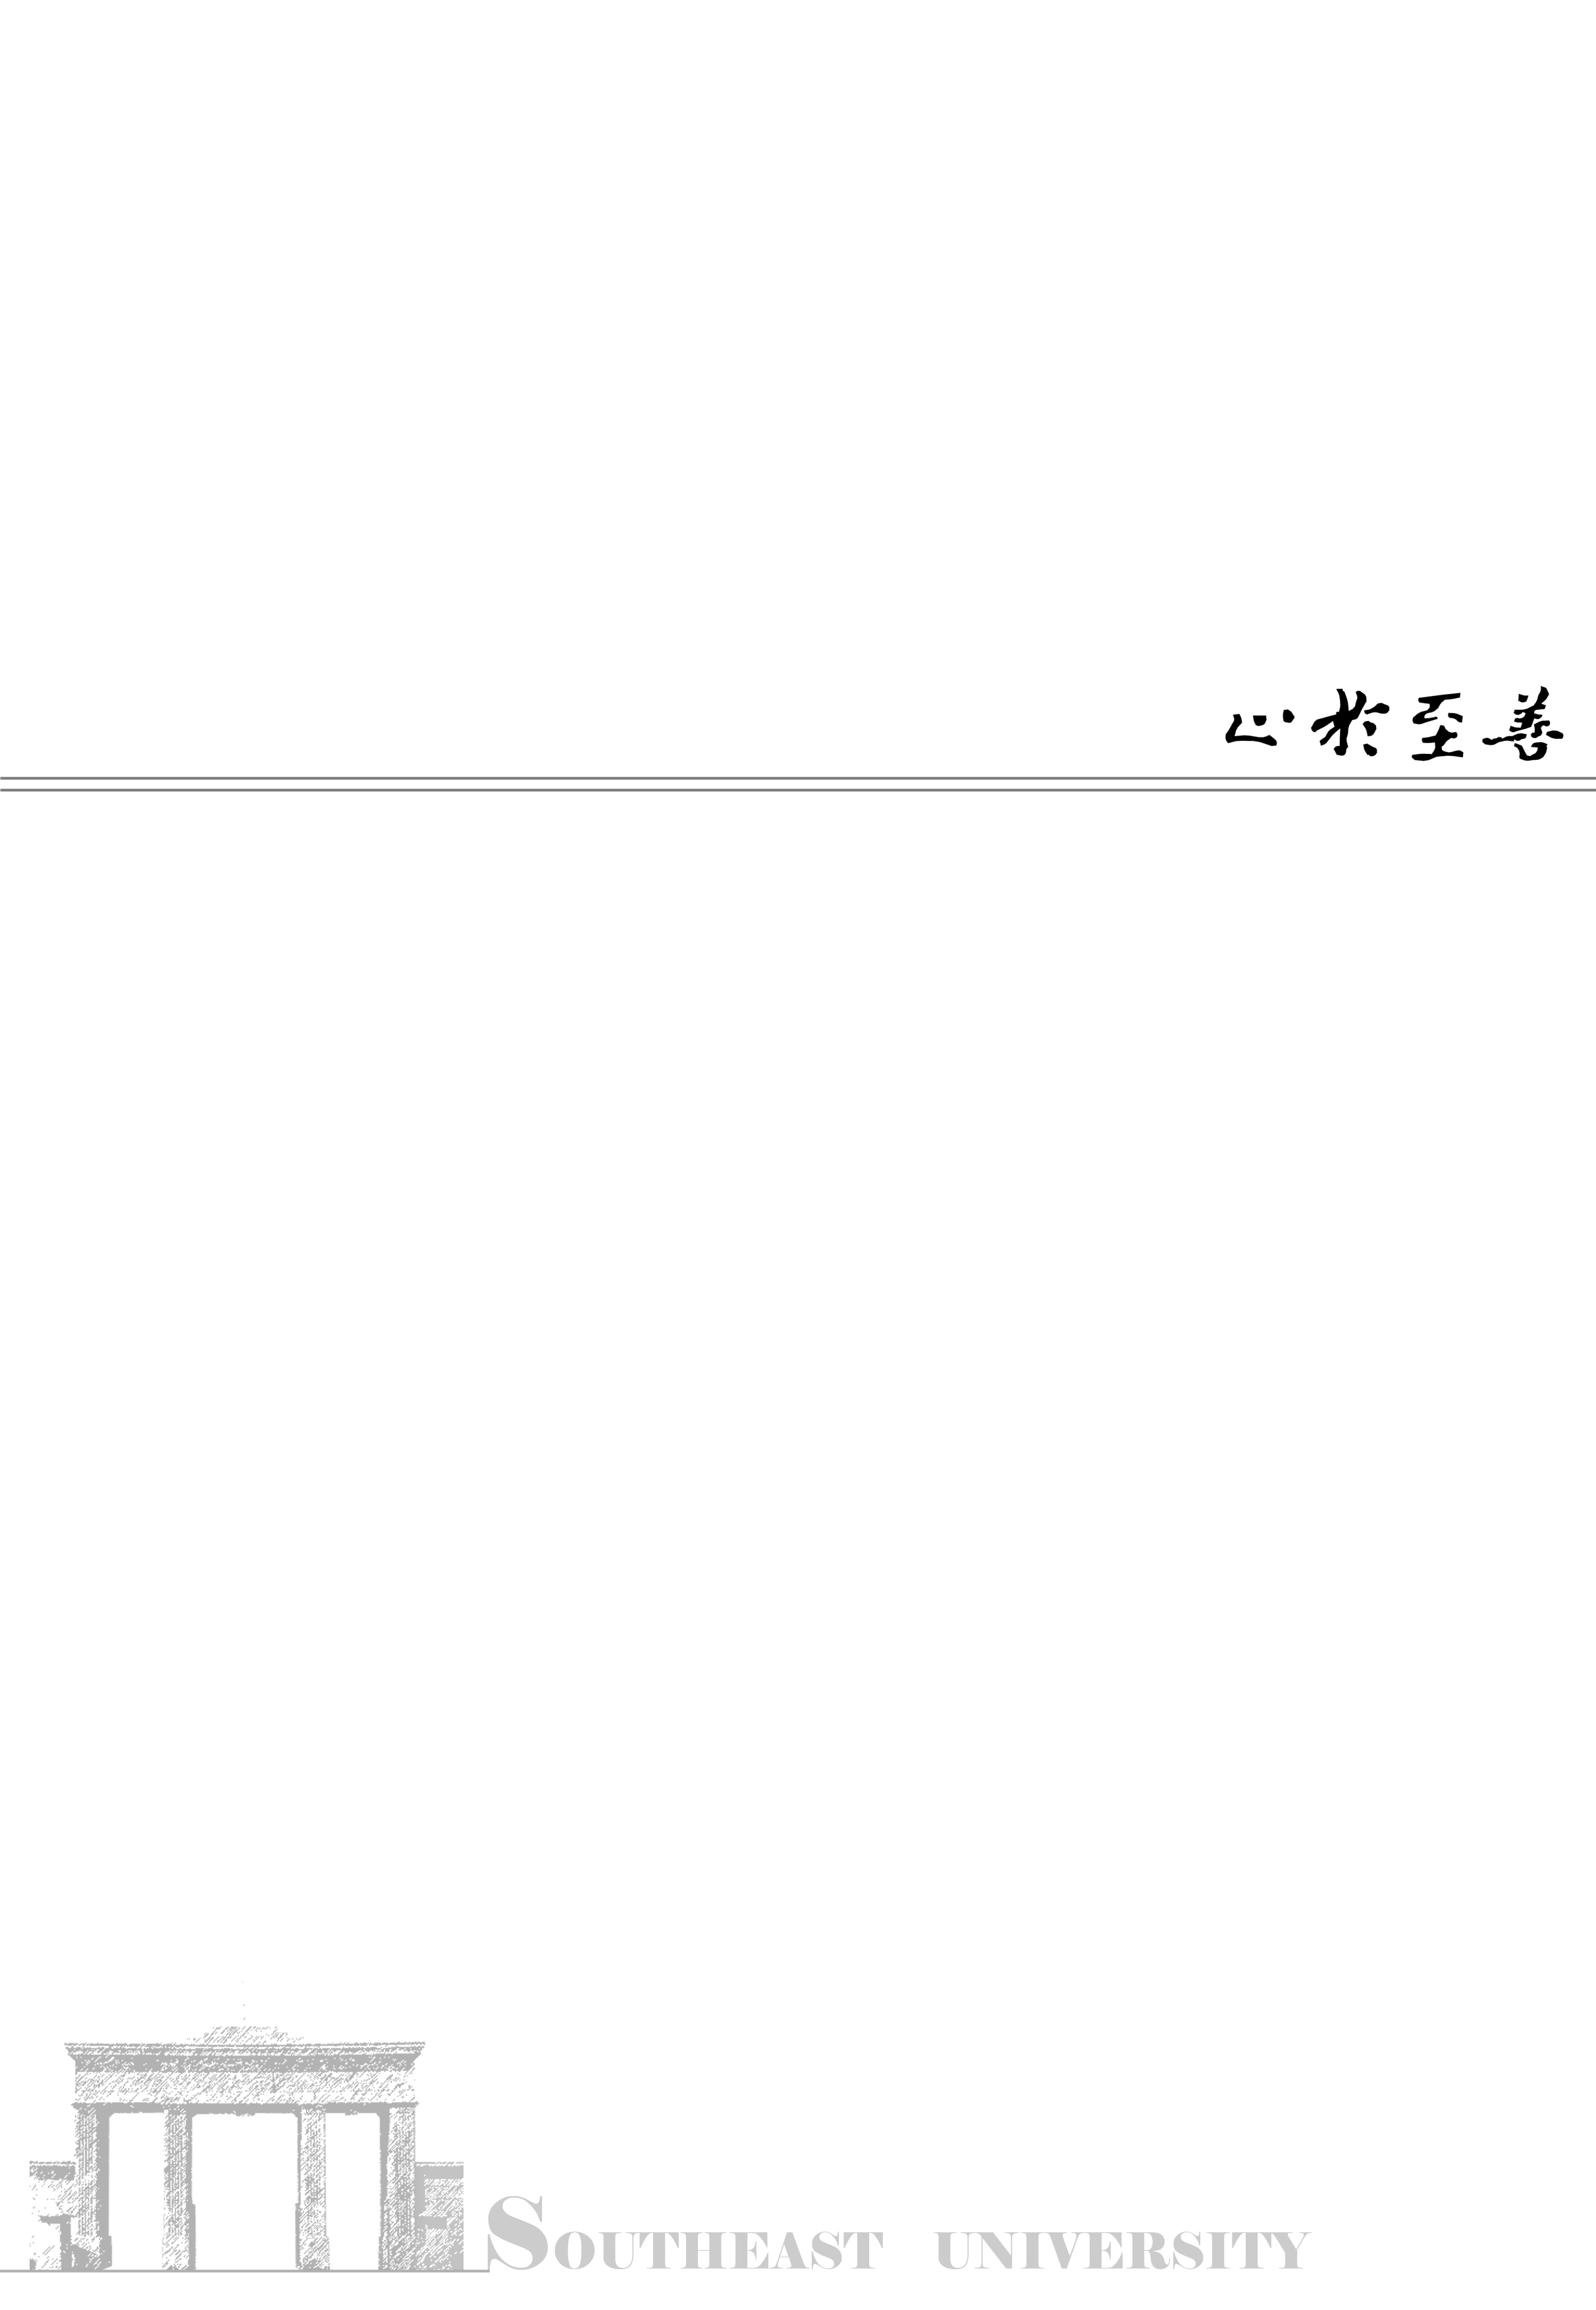
\includegraphics[width=\textwidth]{figures/back-cover.png}
}
\RequirePackage[bottom=1in,left=2.5cm,right=2.5cm,a4paper]{geometry}
\RequirePackage{fancyhdr}
\pagestyle{fancy}
\fancyhf{}
\fancyhead[CO]{\xiaowuhao\universityname{}\@thesistype}
\fancyhead[CE]{ \xiaowuhao\leftmark}
\fancyfoot[CO,CE]{\thepage}
\renewcommand{\headrulewidth}{0.4pt}
\RequirePackage{eso-pic}
\renewcommand{\author}[2]{
 \def\@author{#1}
 \newcommand{\@authoreng}{#2}
}
\newcommand{\@titleeng}{}
\newcommand{\@subtitleeng}{}
\renewcommand{\title}[4]{
 \def\@title{#1}
 \newcommand{\@subtitle}{#2}
 \renewcommand{\@titleeng}{#3}
 \renewcommand{\@subtitleeng}{#4}
}
\newcommand{\@advisorname}{}
\newcommand{\@advisortitle}{}
\newcommand{\@advisornameeng}{}
\newcommand{\@advisortitleeng}{}
\newcommand{\advisor}[4]{
 \renewcommand{\@advisorname}{#1}
 \renewcommand{\@advisortitle}{#2}
 \renewcommand{\@advisornameeng}{#3}
 \renewcommand{\@advisortitleeng}{#4}
}
\newcommand{\@coadvisorname}{}
\newcommand{\@coadvisortitle}{}
\newcommand{\@coadvisornameeng}{}
\newcommand{\@coadvisortitleeng}{}
\newcommand{\coadvisor}[4]{
 \coadvisortrue
 \renewcommand{\@coadvisorname}{#1}
 \renewcommand{\@coadvisortitle}{#2}
 \renewcommand{\@coadvisornameeng}{#3}
 \renewcommand{\@coadvisortitleeng}{#4}
}
\newcommand{\@categorynumber}{}
\newcommand{\categorynumber}[1]{\renewcommand{\@categorynumber}{#1}}
\newcommand{\@secretlevel}{}
\newcommand{\secretlevel}[1]{\renewcommand{\@secretlevel}{#1}}
\newcommand{\@UDC}{}
\newcommand{\UDC}[1]{\renewcommand{\@UDC}{#1}}
\newcommand{\@studentid}{}
\newcommand{\studentid}[1]{\renewcommand{\@studentid}{#1}}
\newcommand\degreetype[2]{\renewcommand\@degreetype{#1}%
\renewcommand\@degreetypeen{#2}}
\newcommand{\@majorlen}{8em}
\newcommand{\@major}{}
\newcommand{\major}[2][8em]{
 \renewcommand{\@majorlen}{#1}
 \renewcommand{\@major}{#2}
}
\newcommand{\@department}{}
\newcommand{\@departmenteng}{}
\newcommand{\department}[2]{
 \renewcommand{\@department}{#1}
 \renewcommand{\@departmenteng}{#2}
}
\newcommand{\@submajor}{}
\newcommand{\submajor}[1]{
 \renewcommand{\@submajor}{#1}
}
\newcommand{\@defenddate}{}
\newcommand{\defenddate}[1]{\renewcommand{\@defenddate}{#1}}
\newcommand{\authorizeorganization}[1]{
 \renewcommand{\@authorizeorganization}{#1}
}

\newcommand{\@authorizedate}{}
\newcommand{\authorizedate}[1]{\renewcommand{\@authorizedate}{#1}}
\newcommand{\@committeechair}{}
\newcommand{\committeechair}[1]{\renewcommand{\@committeechair}{#1}}
\newcommand{\@reviewerA}{}
\newcommand{\@reviewerB}{}
\newcommand{\reviewer}[2]{
 \renewcommand{\@reviewerA}{#1}
 \renewcommand{\@reviewerB}{#2}
}
\newcommand{\CoverTopOption}[3][s]{
 \makebox[1.5cm][#1]{\xiaowuhao #2}:{
   \underline{\makebox[1.5cm][c]{\xiaowuhao #3}}}
}
\newcommand{\CoverBottomOption}[3][4.5cm]{
 \makebox[7cm][s]{
   {\songti\xiaosihao#2} 
   \underline{\makebox[#1][c]{\heiti\xiaosihao#3}} 
 }
}
\newif\ifthanks\thanksfalse
\newcommand\@seuthesisthanks{ }
\newcommand\seuthesisthanks[1]{\renewcommand\@seuthesisthanks{#1}\thankstrue}
\newcommand\@thesisthanks{\ifthanks\thispagestyle{thanksstyle}\fi}
\fancypagestyle{thanksstyle}{%
\fancyhf{}
\fancyfoot[L]{\setlength{\baselineskip}{0pt}%
\rule[-2.5pt]{6cm}{.4pt}\\ \small\@seuthesisthanks}
\renewcommand\headrulewidth{0pt}
}
\newcommand\makebigcover{%generating a3 front cover
\pdfpagewidth=420mm
\pdfpageheight=297mm
\setlength{\paperheight}{297mm}
\setlength{\paperwidth}{420mm}
\thispagestyle{empty}
 \setlength{\unitlength}{1cm}
 \noindent
\begin{picture}(0,0)
\setlength{\unitlength}{1cm}\put(19.5,-8){%

\includegraphics[width=19cm]{figures/front-cover.jpg}}%
\end{picture}
 \begin{picture}(0,0)
\put(19.5,0){
\renewcommand{\arraystretch}{1.0}
   \begin{tabular}{l}
     \CoverTopOption{\schoolcodepre}{\schoolcode} \\
     \CoverTopOption{\categorynumberpre}{\@categorynumber} \\
     \CoverTopOption{\secretlevelpre}{\@secretlevel}\\
     \CoverTopOption{U D C}{\@UDC} \\
     \CoverTopOption{\studentidpre}{\@studentid}
   \end{tabular}
   }
\end{picture}
 \ifengineering
\begin{picture}(0,0)
 \put(23.2,-7.5){ %

\includegraphics[scale=0.65]{figures/engineering.png}}
\end{picture}
   \else \ifmasters
\begin{picture}(0,0)
 \put(24.5,-7.5){ %

\includegraphics[scale=1.1]{figures/master-hwzs.pdf}}
\end{picture}
   \else \ifphd
\begin{picture}(0,0)
 \put(24.5,-7.5){ %

\includegraphics[scale=1.1]{figures/doctor-hwzs.pdf}}
\end{picture}
   \else
   \ClassError{seuthesix}{invalid degree type option.}%
   {Check your class option of degree type to be one of the following:%
   masters, engineering, phd.}
   \fi
   \fi
   \fi
   \begin{picture}(0,0)
 \put(35,0){ %

\includegraphics[width=2cm]{figures/seu-color-logo.png}}
\end{picture}
\begin{picture}(0,0)
 \put(0,-22){ %
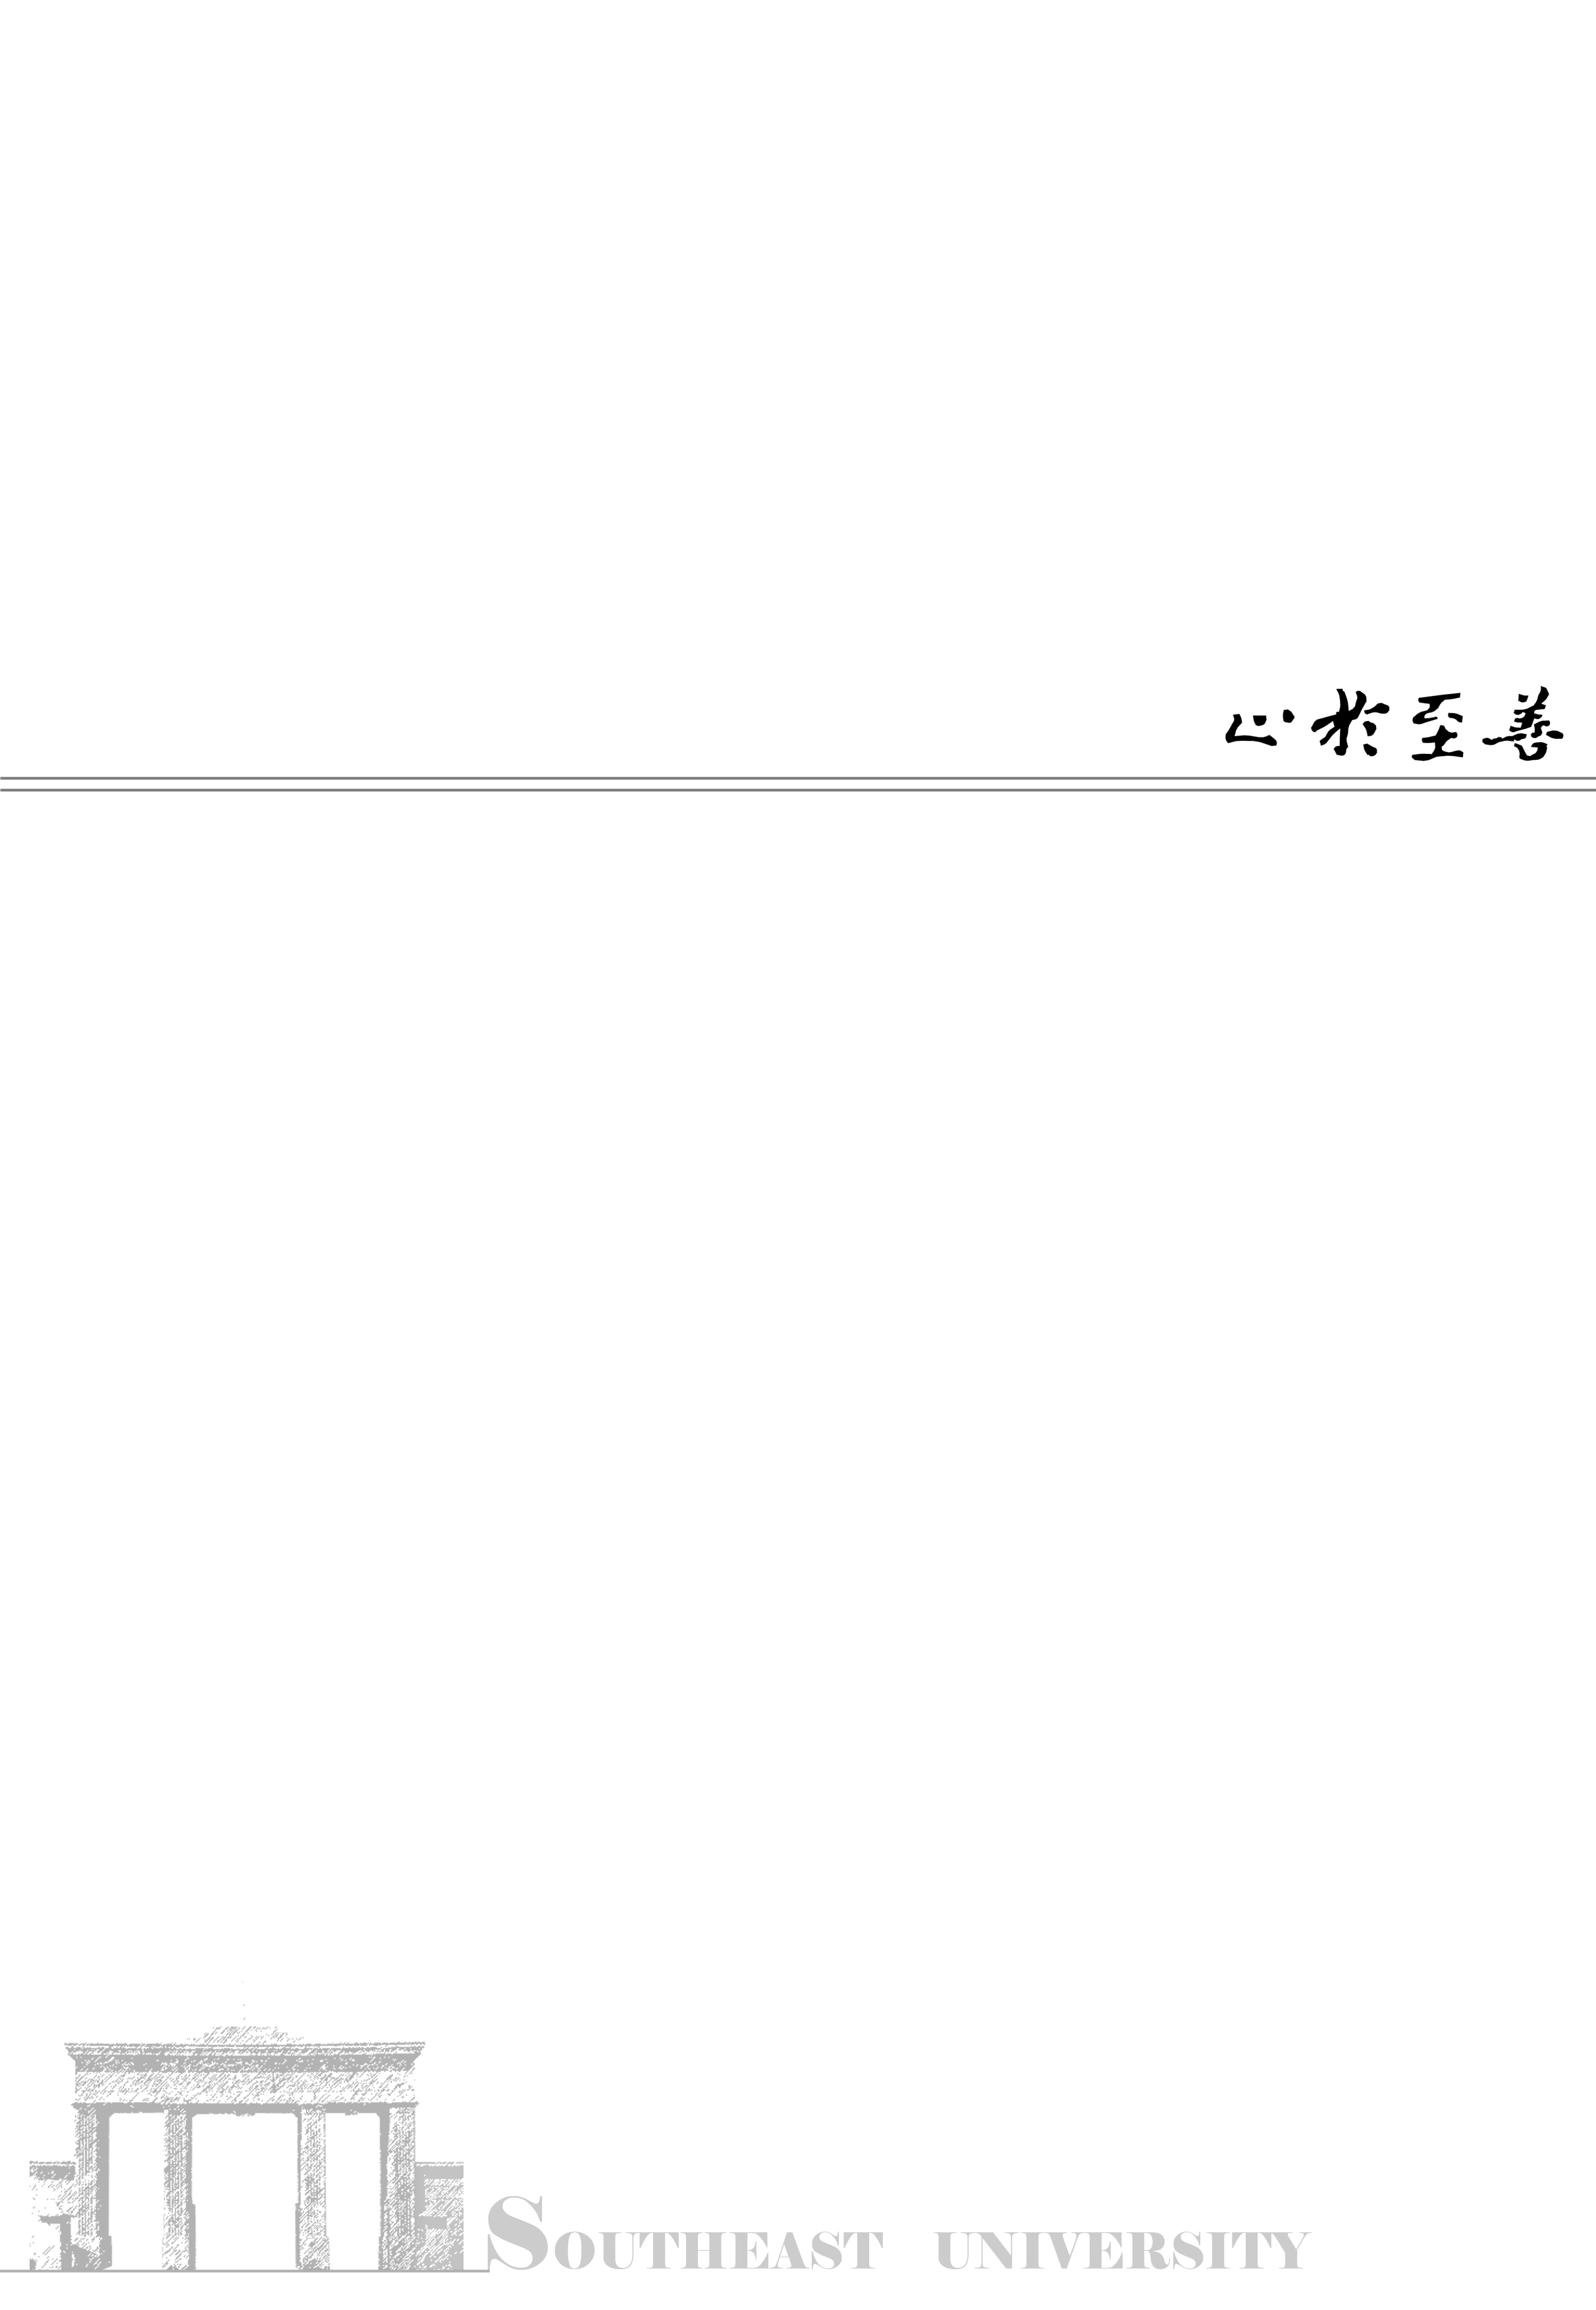
\includegraphics[width=\textwidth]{figures/back-cover.png}}
\end{picture}
\begin{picture}(0,0)
\put(18,-10){%
\parbox[c]{\ccwd}{%
\bfseries%
\setlength{\baselineskip}{0pt}
\@title\\
\rule{0pt}{\ccwd}\\
\@subtitle\\
\vspace*{2cm}
\@author\\
\vspace*{2cm}
\universityname
}
}
\end{picture}

\vspace*{8cm}

\hspace*{20.5cm}
\begin{minipage}{16cm}
   \begin{center}
     \linespread{1.25}
     \yihao\heiti\@title\\
     \yihao\heiti\@subtitle
   \end{center}
\end{minipage}

\hspace*{20.5cm}
\begin{minipage}{16cm}
    \begin{center}
    \setlength{\tabcolsep}{0pt}
    \renewcommand{\arraystretch}{2.0}
     \begin{tabular}{cr}
       \makebox[3.5cm][s]{\xiaoerhao\songti\authorpre: } &
       \underline{\makebox[6cm][s]{
           \hspace*{1cm}
           \makebox[2.5cm][c]{\xiaoerhao\heiti\@author}
           \makebox[2cm][r]{}}} \\
       \makebox[3.5cm][s]{\xiaoerhao\songti\advisorpre: } &
       \underline{\makebox[6cm][s]{
           \hspace*{1cm}
           \makebox[2.5cm][c]{\xiaoerhao\heiti\@advisorname}
           \makebox[2cm][r]{\xiaoerhao\heiti\@advisortitle}}}
       \\
       &
       \ifcoadvisor
       \underline{\makebox[6cm][s]{
           \hspace*{1cm}
           \makebox[2.5cm][c]{\xiaoerhao\heiti\@coadvisorname}
           \makebox[2cm][r]{\xiaoerhao\heiti\@coadvisortitle}}}
       \else
       \fi \\
     \end{tabular}
   \end{center}
  \end{minipage}
   
    \hspace*{20.5cm}
   \begin{minipage}{16cm}
       \begin{center}
   \setlength{\tabcolsep}{10pt}
    \renewcommand{\arraystretch}{2.0}
     \begin{tabular}{ll}
       \CoverBottomOption{\appdegreepre}{\@degreetype} &
       \CoverBottomOption{\authorizeorganizationpre}{\@authorizeorganization} \\
       \CoverBottomOption{\majorpre}{\@major} &
       \CoverBottomOption{\defenddatepre}{\@defenddate}\\
       \CoverBottomOption{\submajorpre}{\@submajor} &
       \CoverBottomOption{\authorizedatepre}{\@authorizedate}\\
       \CoverBottomOption[4.05cm]{\committeechairpre}{\@committeechair} &
       \CoverBottomOption{\reviewerpre}{\@reviewerA}\\
       & \CoverBottomOption{\makebox[2.55cm]{}}{\@reviewerB}
     \end{tabular}
   \end{center}
   \end{minipage}
   
       \vfill
       
       \hspace*{20.5cm}
{\songti\sihao\centerline{\today} \par}
\eject
\pdfpagewidth=210mm
\pdfpageheight=297mm
\setlength{\paperheight}{297mm}
\setlength{\paperwidth}{210mm}
}

\newcommand{\makechinesecover}{
 \hypersetup{
   pdfauthor={\@author},
   pdftitle={\universityname{}\@thesistype},
   pdfsubject={\@title \@subtitle}, 
   pdfcreator={xetex} 
 }

\thispagestyle{empty}
\AddToShipoutPictureFG*{\setlength{\unitlength}{1cm}\put(1,26){%
\renewcommand{\arraystretch}{1.0}
   \begin{tabular}{l}
     \CoverTopOption{\schoolcodepre}{\schoolcode} \\
     \CoverTopOption{\categorynumberpre}{\@categorynumber} \\
     \CoverTopOption{\secretlevelpre}{\@secretlevel}\\
     \CoverTopOption{U D C}{\@UDC} \\
     \CoverTopOption{\studentidpre}{\@studentid}
   \end{tabular}
}
}

\AddToShipoutPictureBG*{\setlength{\unitlength}{1cm}\put(0,22.5){%
\parbox{\paperwidth}{\centering
\includegraphics[width=\paperwidth]{figures/front-cover.jpg}}}}%

   \ifengineering
\AddToShipoutPictureBG*{\setlength{\unitlength}{1cm}\put(0,18){ %
\parbox{\paperwidth}{\centering
\includegraphics[scale=0.65]{figures/engineering.png}}}}%
   \else \ifmasters
\AddToShipoutPictureBG*{\setlength{\unitlength}{1cm}\put(0,18){ %
\parbox{\paperwidth}{\centering
\includegraphics[scale=1.1]{figures/master-hwzs.pdf}}}}%
   \else \ifphd
   \AddToShipoutPictureBG*{\setlength{\unitlength}{1cm}\put(0,18){ %
\parbox{\paperwidth}{\centering
\includegraphics[scale=1.1]{figures/doctor-hwzs.pdf}}}}%
   \else
   \ClassError{seuthesix}{invalid degree type option.}%
   {Check your class option of degree type to be one of the following:%
   masters, engineering, phd.}
   \fi
   \fi
   \fi
\AddToShipoutPictureBG*{\setlength{\unitlength}{1cm}\put(17,27){%
\parbox{\paperwidth}{
\includegraphics[width=2cm]{figures/seu-color-logo.png}}}}%

   \vspace*{8cm}

   \begin{center}
     \linespread{1.25}
     \yihao\heiti\@title\\
     \yihao\heiti\@subtitle
   \end{center}

   \begin{center}
    \setlength{\tabcolsep}{0pt}
    \renewcommand{\arraystretch}{2.0}
     \begin{tabular}{cr}
       \makebox[3.5cm][s]{\xiaoerhao\songti\authorpre: } &
       \underline{\makebox[6cm][s]{
           \hspace*{1cm}
           \makebox[2.5cm][c]{\xiaoerhao\heiti\@author}
           \makebox[2cm][r]{}}} \\
       \makebox[3.5cm][s]{\xiaoerhao\songti\advisorpre: } &
       \underline{\makebox[6cm][s]{
           \hspace*{1cm}
           \makebox[2.5cm][c]{\xiaoerhao\heiti\@advisorname}
           \makebox[2cm][r]{\xiaoerhao\heiti\@advisortitle}}}
       \\
       &
       \ifcoadvisor
       \underline{\makebox[6cm][s]{
           \hspace*{1cm}
           \makebox[2.5cm][c]{\xiaoerhao\heiti\@coadvisorname}
           \makebox[2cm][r]{\xiaoerhao\heiti\@coadvisortitle}}}
       \else
       \fi \\
     \end{tabular}
   \end{center}

   \begin{center}
   \setlength{\tabcolsep}{10pt}
    \renewcommand{\arraystretch}{2.0}
     \begin{tabular}{ll}
       \CoverBottomOption{\appdegreepre}{\@degreetype} &
       \CoverBottomOption{\authorizeorganizationpre}{\@authorizeorganization} \\
       \CoverBottomOption{\majorpre}{\@major} &
       \CoverBottomOption{\defenddatepre}{\@defenddate}\\
       \CoverBottomOption{\submajorpre}{\@submajor} &
       \CoverBottomOption{\authorizedatepre}{\@authorizedate}\\
       \CoverBottomOption[4.05cm]{\committeechairpre}{\@committeechair} &
       \CoverBottomOption{\reviewerpre}{\@reviewerA}\\
       & \CoverBottomOption{\makebox[2.55cm]{}}{\@reviewerB}
     \end{tabular}
   \end{center}
   
   \vfill
   \setcounter{page}{1}
{\songti\sihao\centerline{\today} \par}


 \clearpage\thispagestyle{empty}\cleardoublepage%
 \thispagestyle{empty}
 \begin{center}
   \xiaochuhao
   
   
\includegraphics[height=0.63in]{figures/seu-text-logo}
   
   \ifmasters
   
\includegraphics{figures/master-hwzs}
  \else
  
\includegraphics{figures/doctor-hwzs}
  \fi
  
   \vspace{31.5pt}
   \yihao\heiti\@title\@thesisthanks\\
   \yihao\heiti\@subtitle
  \vspace{42pt}
  
  {
  \setlength{\tabcolsep}{0pt}
   \begin{tabular}{cc}
     \makebox[3.5cm][s]{\xiaoerhao\heiti{}专~~业~~名~~称: } &
     \underline{\makebox[6cm][s]{
         \xiaoerhao\songti\textbf{\@major} }} \\
         \\
       \makebox[3.5cm][s]{ \xiaoerhao\heiti\authorpre:  } &
       \underline{\makebox[6cm][s]{
          \xiaoerhao\songti\textbf{\@author} }} \\
           \\
       \makebox[3.5cm][s]{ \xiaoerhao\heiti\advisorpre:  } &
       \underline{\makebox[6cm][s]{
          \xiaoerhao\songti\textbf{\@advisorname\quad\@advisortitle} }}
\\
       &
       \ifcoadvisor
       \underline{\makebox[6cm][s]{
           \xiaoerhao\songti\textbf{\@coadvisorname\quad\@coadvisortitle} }}
       \else
       \fi 
     \end{tabular}
     }
 \end{center}
}


\newcommand{\makeenglishcover}{%
\clearpage\thispagestyle{empty}\cleardoublepage\thispagestyle{empty}
 \begin{center}
   ~\\
     {\fontsize{24pt}{28pt}\selectfont
       \MakeUppercase{\@titleeng}\\
       \MakeUppercase{\@subtitleeng}
       \par
     }

     \vspace{1.0in}%
     {\fontsize{16pt}{24pt}\selectfont
       {A
       \ifmasters
         Thesis
         \else
         Dissertation
         \fi
       submitted to}\\
       {\universitynameeng}\\
       {For the Academic Degree of \@degreetypeen}\\
       {\vspace{0.5in}}%
       {BY}\\
       {\@authoreng}\\
       {\vspace{0.5in}}%
       {Supervised by:}\\
       {\@advisortitleeng\  \@advisornameeng}\\
       \ifcoadvisor
       {and}\\
       {\@coadvisortitleeng\  \@coadvisornameeng}\\
       \else
       \fi
       {\vspace{0.5in}}%
       {\vfill}
       {\@departmenteng}\\
       {\universitynameeng}\\
       {\todayeng}
       \par
     }%
   \end{center}%

 }

 \newcommand\makecover{%
 \makechinesecover
 \makeenglishcover
 }
 
\renewenvironment{abstract}[1]
{
\pagenumbering{Roman}
\clearpage\thispagestyle{empty}\cleardoublepage\thispagestyle{plain}
 \newcommand{\@keywords}{#1}
 \hypersetup{pdfkeywords={\@keywords}}
 \phantomsection
 \addcontentsline{toc}{chapter}{\@abstracttitle}
   \chapter*{\@abstracttitle}
   \setcounter{page}{1}
}
{
 \par
 \begin{description}
 \item[关键词:] \@keywords
 \end{description}
}

\newenvironment{englishabstract}[1]
{
\cleardoublepage\thispagestyle{plain}
 \newcommand{\@keywords}{#1}
 \phantomsection
 \addcontentsline{toc}{chapter}{Abstract}
	\ctexset{%
chapter/nameformat=\large\bfseries,
chapter/titleformat=\large\bfseries
	}
	  \chapter*{Abstract}
	  	\ctexset{%
chapter/nameformat=\large\heiti,
chapter/titleformat=\large\heiti
	}
}
{
 \par
 \begin{description}
 \item[Keywords:] \@keywords
 \end{description}
}


\newcommand\listofothers{%
\iffigurelist
\cleardoublepage
\phantomsection
\addcontentsline{toc}{chapter}{\listfigurename}
\listoffigures
\fi

\iftablelist
\cleardoublepage
\phantomsection
\addcontentsline{toc}{chapter}{\listtablename}
\listoftables
\fi

\ifalgorithmlist
\cleardoublepage
\phantomsection
\addcontentsline{toc}{chapter}{\listalgorithmname}
\listofalgorithms
\fi

\ifnomlist
\cleardoublepage
\phantomsection
\addcontentsline{toc}{chapter}{\nomname}
\printnomenclature
\fi


}

\newcommand{\mainmatter}{%
\cleardoublepage
\pagenumbering{arabic}
}

\newcommand{\acknowledgement}{%
\cleardoublepage
\phantomsection
\addcontentsline{toc}{chapter}{致 谢}
\chapter*{致 谢}
}

\newcommand{\thesisbib}[1]{%
\bibliographystyle{seuthesix}
\cleardoublepage
\phantomsection
\addcontentsline{toc}{chapter}{\bibname}
\bibliography{#1}
}

\newcommand{\resume}[1]{%
\cleardoublepage
\phantomsection
\addcontentsline{toc}{chapter}{#1}
\chapter*{#1}
}

\newcommand{\seuthesix}{%
 \makebox{S\hspace{-0.3ex}\raisebox{-0.5ex}{E}\hspace{-0.3ex}U\hspace{0.1em}%
 \textsc{Thesix}}
}
\newcommand{\seuthesis}{%
 \makebox{S\hspace{-0.3ex}\raisebox{-0.5ex}{E}\hspace{-0.3ex}U\hspace{0.1em}%
 \textsc{Thesis}}
}
%</class>
%    \end{macrocode}
% \resume{作者简介}
% \seuthesix 开发组,目前仅有四人(当前活跃开发者只有樊智猛一人),希望感兴趣的同学加入。
%\Finale
\endinput
